\documentclass[18pt,oneside,a4paper, titlepage]{article}

\usepackage[hidelinks]{hyperref}
\usepackage[pdftex]{graphicx}

\begin{document}
\begin{figure}[t]
	\centering
	
\includegraphics[scale=0.35]{logo-polimi.png}
\end{figure}
\title{\textbf{TETRIS on STM32F4-Discovery}\\Advanced Operating Systems Project Report\\ A.Y. 2015/2016\\
	Politecnico di Milano}	
\author{Antenucci Sebastiano, matr. 790021\\Cattaneo Michela Gaia, matr. 863116\\Ciceri Filippo, matr. 855162 }
\date{May, 2016}
\maketitle

\newpage
	\tableofcontents

\newpage
\section{Introduction}
	This project aims at implementing the well-known Tetris game on the STM32F429I-Discovery board using Miosix kernel. This board is equipped with:
	\begin{itemize}
		\item high performance ARM Cortex M4 processor with 2D graphics accelerator
		\item 2.4" QVGA TFT LCD display provided with resistive touchscreen
		\item 180Mhz/225 DMIPS execution performance from Flash memory
		\item embedded ST-LINK/V2
	\end{itemize}
	\vspace{1cm}
	\begin{figure}[h]
		\centering
		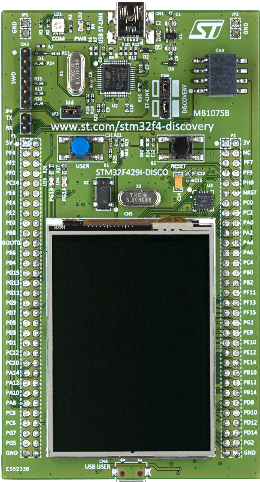
\includegraphics[scale=0.7]{board.jpg}
	\end{figure}
	
\newpage
\section{Tetris game}
	Tetris is a tile-matching puzzle video game.
	\subsection{Gameplay}
		There are seven different pieces of various colors, composed of four square blocks each.\\
		\begin{figure}[h]
			\centering
			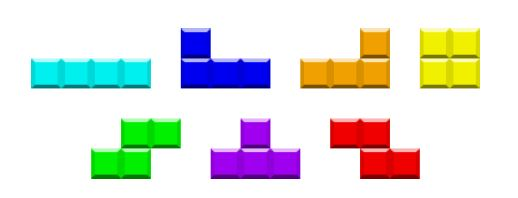
\includegraphics[scale=0.7]{blocks.jpg}
		\end{figure}
		\\
		A random sequence of pieces fall down the playing field and the objective of the game is to translate or rotate the pieces in order to create horizontal lines with no gaps (it is possible to delete more rows simultaneously). When the row is filled, it disappears and any block above gets translated down.\\
		As the game progresses the pieces will not fall faster, as it happens in the classic Tetris game, and there is just one level.\\The game stops when the stack of pieces reaches the top and it is no more possible to add more. 
	\subsection{The game on the board}
		Once the board is connected to power, it displays the starting screen: a touch is expected in order to start a new game.\\
		The LCD display shows the game progress and the touchscreen allows to press the buttons drawn on the bottom of the display in order to translate the current piece or to press the rectangular area in order to rotate the current piece.\\
		The bar at the top of the screen displays the score: 1 point is given when the piece is lied down and 10 points are given when a row is full and canceled.\\
		When it is no more possible to add a new piece on the display, a game over screen will be shown.\\
		In order to start a new game it is necessary to press the reset button.
\newpage
\section{Structure of the program}
	The program is composed of 5 classes, a main (these corresponds to the .cpp files) and 6 .h files.\\
	\vspace{0.5cm}
	\begin{figure}[h]
		\centering
		\includegraphics[scale=0.4]{TetrisClassDiagram.png}
	\end{figure}
	\vspace{0.5cm}
	\\
	\begin{itemize}
		\item[-] The \textbf{Block class} stores the coordinates of the block, its color and its structure.\\
		Block has three different constructors. The classic blocks are created by passing the blockID, a number from 0 to 6, which corresponds to a specific block.
		The blocks used for the "game over" screen are created by passing a character and in order to create a 1x1 piece, useful for the checking functions, it is necessary pass the coordinates to the constructor.\\
		The translate function changes the coordinates of the block, moving it right, left or down, while the rotate method changes its structure, rotating the matrix by 90 degrees.\\
		The deleteRow method is called when it is necessary to delete a row from the structure of the block.\\
		\item[-] The \textbf{Grid class} contains the vector of the blocks that are present in the grid at every iteration and the block composing the "game over" word.\\
		The functions rotate, translate and deleteRow only check if the operation is possible, that is if it does not create a collision, and then call the homonym function of Block.\\
		The addBlock function is the one that creates the blocks and adds them to the grid, it returns true if adding the block does not create a collision, false otherwise. The block is created by passing a random number to the constructor, using the HardwareRng class.\\
		The canAddBlock function make the current piece fall down, by checking if the translation of one unit down is possible first, then performing it. The result of this check is the return value of the function.\\
		\item[-] The \textbf{Movement Draw class} is the class that manages the graphic interface, storing the dimensions of the board and of the components, such as buttons and bars.\\
		The drawStartingScreen draws a black screen with the text "TAP ON THE SCREEN TO START THE GAME!", while drawGameOver draws the ending screen with the "GAME OVER" words written with blocks.\\
		The drawInit delineates the color and the position of the display components: the top bar, the buttons, the arrows in the buttons, the lateral bars and the rectangle of the playing field.\\
		The drawGrid function asks for the blocks present in the grid and draws them one by one, according to their actual position on the field.\\
		
		
		\item[-] The \textbf{Input Manager class} uses threads in order to concurrently listen to touchscreen events.\\
		The waitTouch method creates a thread that waits for a touch on the screen to start the game.\\
		Another thread is created when the game starts, in the startListening function, and it is joined in the gameOver function.\\
		It also has a reference of the grid, in order to apply rotations and translations, according to the input it has received. If the touch cursor is located in the left or right button coordinates, a translation is performed, while, if it is located in the rectangular area of the playing field, a rotation is performed.\\
		The instance of movement draw is necessary to get the correct coordinates of the components and to refresh the screen when an action on the grid is performed.\\
		
		\item[-] The \textbf{Game class} creates the instances of Input Manager, Movement Draw and Grid. It stores the score and updates it at every iteration.\\
		The startGame function manages a single game. It calls the Movement Draw methods to display the starting screen, the components and the grid when necessary. It also handles the inputs, with the support of mutexes, and the grid updates and checks.
	\end{itemize}

\newpage

\section{Key Parts of the Program and their Interaction}
	This section briefly describes the major implementations made in order to best model the game.
	\subsection{Dynamic Grid Computation}
		Due to choices made with the formation of the grid, we didn't have an array to represent our grid to continuously update. This wasn't much of an issues, since due to the 
		structure of our grid we could compute every time we would need it in the program. With the way we designed it all, the only time we would need for the grid to be dynamically 
		computed was when we were looking for collisions.
	\subsection{Collision detection}
		This is probably the most important backend method made. It is called every time a piece has to move, be it simple downward advancement, lateral movements or rotation. Fundamentally,
		this method checks if the block in its new position will collide with any blocks in the already existing grid. Note that every time this method is called, it is preceded by the creation of a new 
		block, and usually even by the removal of a block from the grid if it is being tested. \\
		The way the method works is by first computing the "static" grid, matching it to an array of 1's and 0's. Consequently, it adds the "new" block to the grid, by summing it on top of the
		computed grid. As a result, any overlaps between the already placed pieces and the new one will result in a 2 on the grid. The method checks for any 2's in the grid, and returns a collision
		if a 2 is found, false otherwise. This can be exploited for pretty much any check the game has to make, from simple rotations and movements, as well as the removal of complete rows.
	\subsection{Row Deletion and Points}
		While the checks for rotation or movement are simple, row deletion was a little more challenging. In order to detect a collision, we had to check a whole line in one iteration. In order to do this,
		we create an array of 13 lines, one for each line of the grid. Then, for every line, we iterate on each column. On each iteration, we create a small 1x1 block, in the current line and column, and
		check whether this creates a collision. If there is a collision, we increase the counter for the line. By checking every column of a line once, if there is a collision in each column, we will see
		that the entry representing the line in the temporary array will be equal to the Grid's number of columns, defined as GRIDX in our code. \\
		Once each line has been tested, we check the array that condenses every line into a value. Upon the first occurrence of the maximum value of GRIDX, the row deletion algorithm deletes the first row
		it finds from every block that contains it, and moves all blocks above the current row down by 1. Afterwards, it terminates and returns true. This is used both as a visual aid, so that each row can
		be seen deleted one-by-one, as well as simplifying the deletion of rows, by doing one at a time instead of deleting multiple rows in bulk. Every time the row deletion algorithm returns true, it is called
		again and it once again check all rows using the procedure previously described, and it continues getting called until no new rows can be deleted. At that point, it will return false, and a new block 
		will be added to the game.
	\subsection{Vector Cleanup}
		Another problem that arises with the way our grid is structured is that the blocks vector may contain numerous empty blocks. In order to prevent this, every time a row is deleted,
		all blocks are checked for emptiness. If one block is empty, it is removed from the vector by using the Vector.erase() method. Once a block is deleted, the method is called again, much like
		in the case of row deletion, since sequential deletion is simpler than bulk deletion.
	\subsection{Synchronization of Input and Movement}
		Since the game is composed fundamentally by two threads, one handling inputs and the other handling everything else, synchronizing the two was an issue. For example, sometime the game would start
		before the input manager was up and running, and the first two movements would fire before the inputs were read. In order to avoid this, we used the mutex structure with condition variables, and made
		the game start only after an input is read. \\
		The other major issue was movements happening during row deletion or right inbetween the addition of a new block to the game. To avoid this, we added a new global boolean variable onEnd, which tells us
		whether or not the last block has yet reached its bottom-most position, and can therefore no longer move. The variable is set to true every time a new block is added, meaning that the block can be freely
		moved by user inputs, while it is set to false the moment the row deletion checks begin. This makes it so that the blocks don't get moved or rotated into funky positions after they are placed into their 
		final position.
	\subsection{The Screen}
		In order to represent the different blocks we decided to draw them dynamically: we represent each block in a 4x4 integer (1, 0) matrix, so we can 
		display them simply drawing every elementary part of the block (a small square).
		In this way we are able to display all the blocks with only one function and also to draw text like the "Game Over" screen simply adding new type of blocks.
		For displaying the left right arrow button we manually drew the arrow with the line function of MxGui then we surrounded them with a square to represent the border of the button.
		We also drew another square which is displayed only when the button is pressed to graphically simulate the button pressed.
		We decided to insert two side bars in order to adjust the dimension of the game grid and also to fit the original layout of the game.
	% To manage the imput we decide to use a separated thread from the pthread class in order to allaw the user to perform tranlsate and rotation while the main thread  handles the fall of the block and performs all of the checks like collision and delete row. The InputManager thread wait for the touch event and then perform the related action (translate dx, translate sx and rotate). To correctly interpretate wher the touch event happends, we check the top left and bottom right coordinates of every button with coordinates of the event so we can establish which botton has been pressed by the user. To manage concurrency between InputManager and main thread we used mutex of sync.h class from miosix kernel.
	

\newpage
\section{Future possible implementation}
% problems/possible future impl:
%	- the levels and the growing speed of the fall
%	- the probability of the blocks
%	- the more performant draw of the screen
	We wanted to point out that our Tetris implementation works on the board with the rules presented in the second section.\\
	Even if the gameplay does not really differ from the classic game, it is missing the implementation of the different levels and the growing speed of the fall of the pieces. This can be considered a future possible implementation, that we did not consider crucial for the game.\\
	Another future possible implementation can be the one regarding the probability of the block occurrence. The blocks are added randomly to the playing field and it can happen that the same piece type is added to the grid two or three times in a row. This can be improved by decreasing the chance of the block occurrence if a block of the same structure has just been added, so that blocks not recently added have a better chance to be chosen.\\
	Moreover we have not handled any improvement in the drawing performance. It is not really important for the game experience, but, when there are several blocks to be drawn on the playing field, the display flickers a little bit. This could be fixed by managing the drawing of the blocks with a thread that refreshes more frequently the display.
	
\newpage
\section{Software and tool used}
	\begin{itemize}
		\item \textbf{miosix-kernel}: OS kernel designed to run on 32bit microcontrollers. (\url{https://miosix.org/})
		\item \textbf{mxgui}: Miosix GUI library.
		\item \textbf{Notepad++}: to write the code.
		\item \textbf{QSTlink2}: to transfer the program to the board. (\url{https://github.com/fpoussin/qstlink2})
	\end{itemize}

\end{document}